
%%%%%%%%%%%%%%%%%%%%%%% file typeinst.tex %%%%%%%%%%%%%%%%%%%%%%%%%%%%%%
%
% This is the LaTeX source for the instructions to authors using
% the LaTeX document class SVMultln with class option 'lnicst'
% for contributions to the Lecture Notes of the Institute for
% Computer Sciences, Social-Informatics and
% Telecommunications Engineering series.
% www.springer.com/series/XXXX       Springer Heidelberg 2007/08/05
%
% It may be used as a template for your own input - copy it
% to a new file with a new name and use it as the basis for
% your article. It contains a few tweaked sections to demonstrate
% features of the package, though.
%
% If you have not much experiences with Springer LaTeX support,
% you should better use the special demonstration file "lnicst.tex"
% included in the LaTeX package for LNICST as template.
%
%%%%%%%%%%%%%%%%%%%%%%%%%%%%%%%%%%%%%%%%%%%%%%%%%%%%%%%%%%%%%%%%%%%%%%%%

\documentclass[lnicst,sechang,a4paper]{svmultln}
\usepackage{amssymb}
\setcounter{tocdepth}{3}
\usepackage{graphicx}
\usepackage{bbding}

\usepackage{url}
\urldef{\mailsa}\path|boliangzai@foxmail.com,djhe@sei.ecnu.edu.cn|
\usepackage[pdfpagelabels,hypertexnames=false,breaklinks=true,bookmarksopen=true,bookmarksopenlevel=2]{hyperref}

\begin{document}

\mainmatter  % start of an individual contribution

% first the title is needed
\title{A light-weight secure protocol for small data dissemination in WSNs}

% a short form should be given in case it is too long for the running head
\titlerunning{a light-weight secure protocol}

% the name(s) of the author(s) follow(s) next
%
% NB: Chinese authors should write their first names(s) in front of
% their surnames. This ensures that the names appear correctly in
% the running heads and the author index.
%
\author{Yan Wang%
%\thanks{Please note that the LNICST Editorial assumes that all authors have used
%the western naming convention, with given names preceding surnames. This determines
%the structure of the names in the running heads and the author %index.}%
, Daojing He \Envelope
}  %
\authorrunning{Yan Wang et al.}
% (feature abused for this document to repeat the title also on left hand pages)

% the affiliations are given next
\institute{East China Normal University,\\
3663 N, Zhongshan Rd,Putuo District, Shanghai,China\\
\mailsa
%\\
%\url{http://www.springer.com/series/7911}
}

%
% NB: a more complex sample for affiliations and the mapping to the
% corresponding authors can be found in the file "lnicst.dem",
% that is contained in the LNICST LaTeX support package.
%

\toctitle{Lecture Notes in Business Information Processing}
\tocauthor{Authors' Instructions}
\maketitle


\begin{abstract}


This paper argues for a security scheme for security of data dissemination discovery and dissemination in WSNs, Wireless sensor networks. Our scheme is designed to be simple as well as has little impact on memory consumption and network traffic. The scheme is designed in light of issues derived from many different kinds of attacks.

\keywords{Data discovery and dissemination, Security, Wireless sensor networks, Efficiency}
\end{abstract}
\section{Introduction}

WSN consists of a lot of space-distributed sensors. To function a specific application,such as health-care, or obtain valuable information about physical world, Network manager needs every node work together though wireless channel.

As shown in Fig.1. Normally, WSNs collect data to a prime location named a base station. Base station could be your computer which allows network manager to store and analyse collected data later. On the other hand, each powerful sensor node has several parts, a circuit which is able to be interfaced with other devices, a battery for supplying electrical power, a radio transceiver.Actually, WSNs are usually deployed in hostile or remote area with many kinds of topology, such as ring, star. 

Obviously, it is very important that a message should be protected from vicious attackers. And broadcast authentication is a very common security mechanism in WSNs, since broadcast authentication is able to provide message with confidentiality and authentication. 

WSN is one of the major milestones in the field of communication. These networked collection of nodes take us a step closer to obtaining valuable about the physical world. WSN are used popularly in many applications like remote control and monitoring, construction safety systems, environmental monitoring, health care management, disaster management, srveilance operations, smart homes, habitat monitoring, indoor sensor networks, seismic monitoring of buildings etc[1].

However, we argue every WSN, running any application, should be able to present hunman manager the ability to determine whether the WSN is functioning or not.

Why drip is reliable?
Drip provides a transport-layer interface to multiple channels of reliable message dissemination. Each component wishing to use Drip registers a specific identifier, which represents a reliable dissemination channel. Message received on that channel will be delivered directly to the component.

But it does introduce extra complexity for a component that has several independetn variables which must be reliably synchronized among all nodes in the networks.
Wireless sensor networks is usually deployed in outdoor environment, especially hostile environment to collect sensitive information. In battlefield. an adversary is able to inject vicious code images and take control of the entire WSNs.

Since an administrator of a Wireless Sensor networks often reconfigures, queries and reprograms a WSNs, The above functions can be provided by dissemination protocol, which is used to deliver some small data, such as two-byte configuration parameters, to every node in networks.

The small dissemination protocols add, delete, and modify these data by requesting each node exchange their stored data and eventually reach consistency over the networks.

Consistency is the unique property of small dissemination protocol, making a whole WSN be immune to packet loss. A disconnected one also can get latest data image from neighbor nodes.

Although reliability is necessary for dissemination protocol, it makes networks robust to temporary disconnection and high packet loss, but We cannot lay too much emphasis on the importance of security.However, to the best of our knowledge, all existing data discovery and dissemination protocols only address reliable data transmission, but provide no security mechanism.

Among existing dissemination protocols, Drip, Dip, and DHV are the most well known and widely used. These three protocols are all included in TinyOS distributions.

We first investigate the requirements for a secure broadcast mechanism in smart grids, and then show some security weakness and efficiency problems of existing broadcast authentication mechanisms.
1)We firstly investigate the security problem in data discovery and dissemination protocol of WSNs and indicate the lack of authentication of disseminated data refers to a vulnerability. The energy in each sensor node is supplied by limited battery power or its energy harvesting capacity, thus it is significant to maintain energy to lengthen the operational lifetime of a sensor node.

\section{Network, Trust And Threat Models}
As shown in Fig. 1(b), Wsns consists of a lot of distrubited sensor nodes, manys network users and only a owner. This is a very simple and easy structure. The network uses use mobile devices such as PDAs and mobile phone to control the whole WSNs. The Network owner may be off-line, who has bootstrapped the keying materials for the mobile devices to enforce reprogramming privilege policy. It is assumed that the owner cannot be compromised by enemy or attacker and still has some capability of doing some computation and judgement, such as hash operation and  a lot of other cryptography techniques. We assume Deluge as the underlying code dissemination protocol. We also assume sensor nodes, for example using the scheme of [19]. To enable each node to check whether the subscription period of each authorize user has expired, we assume there is a loose time synchronization among the nodes with the help of some existing secure time synchronization scheme.
We assume there is a loose time synchronization among the nodes with the help of some existing secure time synchronization scheme.



\section{Checking the PDF File}

Kindly assure that the Contact Publication Chair is given the name and email
address of the contact author for your paper. The Contact Publication Chair
uses these details to compile a list for our production department at
SPS in India. Once the files have been worked upon, SPS sends a copy of
the final pdf of each paper to its contact author. The contact author is
asked to check through the final pdf to make sure that no errors have
crept in during the transfer or preparation of the files. This should
not be seen as an opportunity to update or copyedit the papers, which is
not possible due to time constraints. Only errors introduced during the
preparation of the files will be corrected.

This round of checking takes place about two weeks after the files have
been sent to the Editorial by the Contact Publication Chair, i.e., roughly
seven weeks before the start of the conference for conference
proceedings, or seven weeks before the volume leaves the printer's, for
post-proceedings. If SPS does not receive a reply from a particular
contact author, within the timeframe given, then it is presumed that the
author has found no errors in the paper. The tight publication schedule
of LNICST does not allow SPS to send reminders or search for alternative
email addresses on the Internet.

In some cases, it is the Contact Publication Chair that checks all the final
pdfs. In such cases, the authors are not involved in the checking phase.

\subsection{Additional Information Required by the Publication Chair}

%When sending your final files, please include a readme informing the
%Contact Publication Chair which of your names is/are your first name(s) and
%which is/are your family name(s). This is particularly important for
%Spanish and Chinese names. Authors are listed alphabetically according
%to their surnames in the author index.
If you have more than one surname, please make sure that the Publication Chair
knows how you are to be listed in the author index.

\subsection{Copyright Forms}

LNICST has integrated its copyright form into the paper submission system
which means that you must agree with transferring the copyrights of your
paper while uploading your camera ready version to the submission system.
The author who uploads the paper should be the author who has the authority
to agree with the terms of the copyright agreement on behalf of all the
authors. After confirming the agreement the author will receive an e-mail
with the filled document which is confirmed by both the author and ICST.

\section{Paper Preparation}

Springer
provides you with a complete integrated \LaTeX{} document class (\texttt{SVMultln.cls})
for multi-author books and the associated class option file (\texttt{svlnicst.clo})
to get the layout for the LNICST series.
Papers not complying with the LNICST style will be reformatted. This can
lead to an increase in the overall number of pages. We would therefore
urge you not to squash your paper.

Please always cancel any superfluous definitions that are
not actually used in your text. If you do not, these may conflict with
the definitions of the macro package, causing changes in the structure
of the text and leading to numerous mistakes in the proofs.

If you wonder what \LaTeX{} is and where it can be obtained, see the
``\textit{LaTeX project site}'' (\url{http://www.latex-project.org})
and especially the webpage ``\textit{How to get it}''
(\url{http://www.latex-project.org/ftp.html}) respectively.

When you use \LaTeX\ together with our document class file,
\texttt{SVMultln.cls} and the documentclass option \texttt{lnicst},
your text is typeset automatically in Computer Modern Roman (CM) fonts.
Please do
\emph{not} change the preset fonts. If you have to use fonts other
than the preset fonts, kindly submit these with your files.

Please use the commands \verb+\label+ and \verb+\ref+ for
cross-references and the commands \verb+\bibitem+ and \verb+\cite+ for
references to the bibliography, to enable us to create hyperlinks at
these places.

For preparing your figures electronically and integrating them into
your source file we recommend using the standard \LaTeX{} \verb+graphics+ or
\verb+graphicx+ package. These provide the \verb+\includegraphics+ command.
In general, please refrain from using the \verb+\special+ command.

Remember to submit any further style files and
fonts you have used together with your source files.

\subsubsection{Headings.}

Headings should be capitalized
(i.e., nouns, verbs, and all other words
except articles, prepositions, and conjunctions should be set with an
initial capital) and should,
with the exception of the title, be aligned to the left.
Words joined by a hyphen are subject to a special rule. If the first
word can stand alone, the second word should be capitalized.

Here are some examples of headings: ``Criteria to Disprove
Context-Freeness of Collage Language", ``On Correcting the Intrusion of
Tracing Non-deterministic Programs by Software", ``A User-Friendly and
Extendable Data Distribution System", ``Multi-flip Networks:
Parallelizing GenSAT", ``Self-determinations of Man".

\subsubsection{Lemmas, Propositions, and Theorems.}

The numbers accorded to lemmas, propositions, and theorems, etc. should
appear in consecutive order, starting with Lemma 1, and not, for
example, with Lemma 11.

\subsection{Figures}

For \LaTeX\ users, we recommend using the \emph{graphics} or \emph{graphicx}
package and the \verb+\includegraphics+ command.

Please check that the lines in line drawings are not
interrupted and are of a constant width. Grids and details within the
figures must be clearly legible and may not be written one on top of
the other. Line drawings should have a resolution of at least 800 dpi
(preferably 1200 dpi). The lettering in figures should have a height of
2~mm (10-point type). Figures should be numbered and should have a
caption which should always be positioned \emph{under} the figures, in
contrast to the caption belonging to a table, which should always appear
\emph{above} the table; this is simply achieved as matter of sequence in
your source.

Please center the figures or your tabular material by using the \verb+\centering+
declaration. Short captions are centered by default between the margins
and typeset in 9-point type (Fig.~\ref{fig:example} shows an example).
The distance between text and figure is preset to be about 8~mm, the
distance between figure and caption about 6~mm.

To ensure that the reproduction of your illustrations is of a reasonable
quality, we advise against the use of shading. The contrast should be as
pronounced as possible.

If screenshots are necessary, please make sure that you are happy with
the print quality before you send the files.
\begin{figure}
\centering
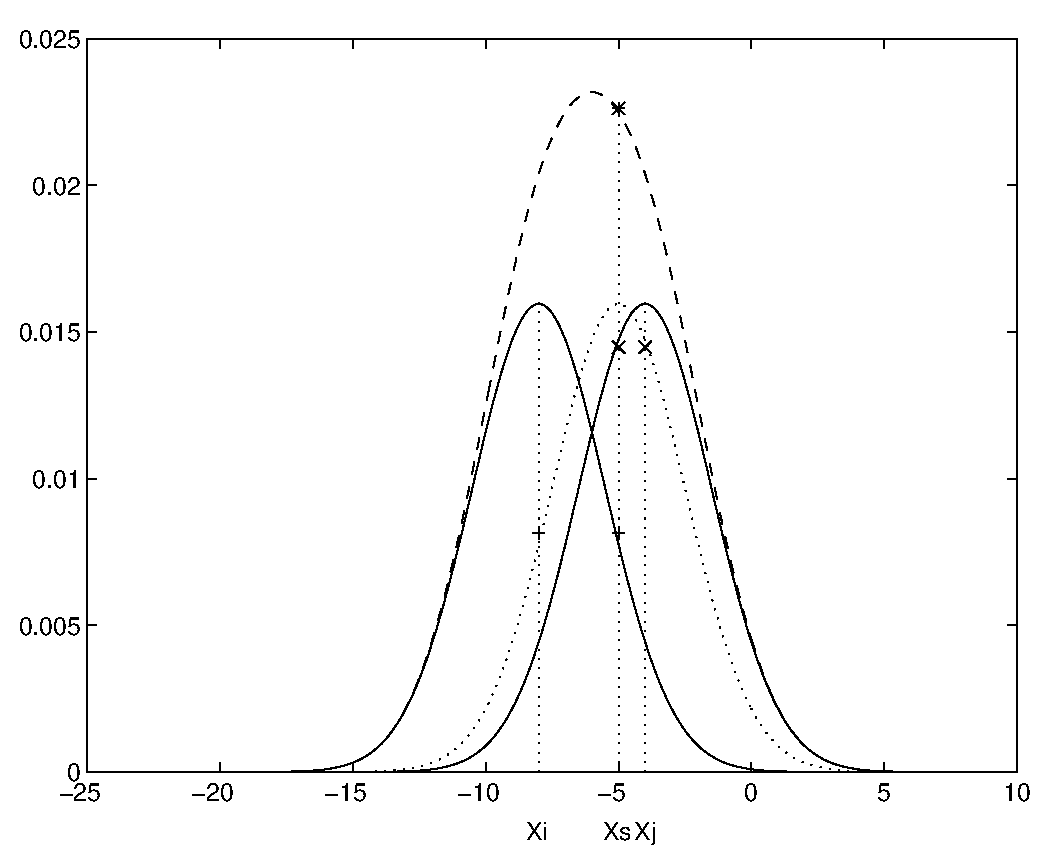
\includegraphics[height=6.2cm]{eijkel2}
\caption{One kernel at $x_s$ (\emph{dotted kernel}) or two kernels at
$x_i$ and $x_j$ (\textit{left and right}) lead to the same summed estimate
at $x_s$. This shows a figure consisting of different types of
lines. Elements of the figure described in the caption should be set in
italics, in parentheses, as shown in this sample caption.}
\label{fig:example}
\end{figure}

Please define figures (and tables) as floating objects. Please avoid
using optional location parameters like ``\verb+[h]+" for ``here".

\paragraph{Remark 1.}

In the printed volumes, illustrations are generally black and white
(halftones), and only in exceptional cases, and if the author is
prepared to cover the extra cost for color reproduction, are colored
pictures accepted. Colored pictures are welcome in the electronic
version free of charge. If you send colored figures that are to be
printed in black and white, please make sure that they really are
legible in black and white. Some colors as well as the contrast of
converted colors show up very poorly when printed in black and white.

\subsection{Formulas}

Displayed equations or formulas are centered and set on a separate
line (with an extra line or halfline space above and below). Displayed
expressions should be numbered for reference. The numbers should be
consecutive within each section or within the contribution,
with numbers enclosed in parentheses and set on the right margin --
which is the default if you use the \emph{equation} environment, e.g.
\begin{equation}
  \psi (u) = \int_{o}^{T} \left[\frac{1}{2}
  \left(\Lambda_{o}^{-1} u,u\right) + N^{\ast} (-u)\right] dt \;  .
\end{equation}

Please punctuate a displayed equation in the same way as ordinary
text but with a small space before the end punctuation.

\subsection{Footnotes}

The superscript numeral used to refer to a footnote appears in the text
either directly after the word to be discussed or -- in relation to a
phrase or a sentence -- following the punctuation sign (comma,
semicolon, or period). Footnotes should appear at the bottom of
the
normal text area, with a line of about 2~cm set
immediately above them.\footnote{The footnote numeral is set flush left
and the text follows with the usual word spacing.}

\subsection{Program Code}

Program listings or program commands in the text are normally set in
typewriter font, e.g., CMTT10 or Courier.

\medskip

\noindent
{\it Example of a Computer Program}
\begin{verbatim}
program Inflation (Output)
  {Assuming annual inflation rates of 7%, 8%, and 10%,...
   years};
   const
     MaxYears = 10;
   var
     Year: 0..MaxYears;
     Factor1, Factor2, Factor3: Real;
   begin
     Year := 0;
     Factor1 := 1.0; Factor2 := 1.0; Factor3 := 1.0;
     WriteLn('Year  7% 8% 10%'); WriteLn;
     repeat
       Year := Year + 1;
       Factor1 := Factor1 * 1.07;
       Factor2 := Factor2 * 1.08;
       Factor3 := Factor3 * 1.10;
       WriteLn(Year:5,Factor1:7:3,Factor2:7:3,Factor3:7:3)
     until Year = MaxYears
end.
\end{verbatim}
%
\noindent
{\small (Example from Jensen K., Wirth N. (1991) Pascal user manual and
report. Springer, New York)}

\subsection{Citations}

%The list of references is headed ``References" and is not assigned a
%number. The list should be set in small print
%and placed at the end of your contribution, in front of the appendix,
%if one exists.
%Please do not insert a pagebreak before the list of references if the
%page is not completely filled.
%An example is given at the
%end of this information sheet.
For citations in the text please use
square brackets and consecutive numbers: \cite{jour}, \cite{lnicstchap},
\cite{book}, \cite{proceeding1} -- provided automatically
by \LaTeX 's \verb|\cite| \dots\verb|\bibitem| mechanism.

\subsection{Page Numbering and Running Heads}

There is no need to include page numbers. If your paper title is too
long to serve as a running head, it will be shortened. Your suggestion
as to how to shorten it would be most welcome.

\section{LNICST Online}

The online version of the volume will be available in LNICST Online.
Members of institutes subscribing to the Lecture Notes in Business Information
Processing series have access to all the pdfs of all the online
publications. Non-subscribers can only read as far as the abstracts. If
they try to go beyond this point, they are automatically asked, whether
they would like to order the pdf, and are given instructions as to how
to do so.

\section{BibTeX Entries}

The correct BibTeX entries for the Lecture Notes in Computer Science
volumes can be found at the following Website shortly after the
publication of the book:
\url{http://www.informatik.uni-trier.de/~ley/db/journals/lncs.html}

\subsubsection*{Acknowledgments.} The heading should be treated as a
subsubsection heading and should not be assigned a number.

\section{Advances in References}\label{references}

In order to permit cross referencing within LNCS/LNICST-Online, and eventually
between different publishers and their online databases, LNCS/LNICST will
be standardizing the format of the references. This
feature will increase the visibility of publications and facilitate
academic research considerably. Please base your references on the
examples below. References that don't adhere to this style will be
reformatted by Springer. You should therefore check your references
thoroughly when you receive the final pdf of your paper.
The reference section must be complete. You may not omit references.
Instructions as to where to find a fuller version of the references are
not permissible.

The following section shows a sample LNCS/LNICST reference list with 6 entries for
journal articles \cite{jour}, a LNCS/LNICST chapter \cite{lnicstchap}, a book
\cite{book}, proceedings without editors \cite{proceeding1} and
\cite{proceeding2}, as well as an URL \cite{url}.
Please note that proceedings published in LNICST are not cited with their
full titles, but with their acronyms!

\begin{thebibliography}{4}

\bibitem{jour} Smith, T.F., Waterman, M.S.: Identification of Common Molecular
Subsequences. J. Mol. Biol. 147, 195--197 (1981)

\bibitem{lnicstchap} May, P., Ehrlich, H.C., Steinke, T.: ZIB Structure Prediction Pipeline:
Composing a Complex Biological Workflow through Web Services. In: Nagel,
W.E., Walter, W.V., Lehner, W. (eds.) Euro-Par 2006. LNCS, vol. 4128,
pp. 1148--1158. Springer, Heidelberg (2006)

\bibitem{book} Foster, I., Kesselman, C.: The Grid: Blueprint for a New Computing
Infrastructure. Morgan Kaufmann, San Francisco (1999)

\bibitem{proceeding1} Czajkowski, K., Fitzgerald, S., Foster, I., Kesselman, C.: Grid
Information Services for Distributed Resource Sharing. In: 10th IEEE
International Symposium on High Performance Distributed Computing, pp.
181--184. IEEE Press, New York (2001)

\bibitem{proceeding2} Foster, I., Kesselman, C., Nick, J., Tuecke, S.: The Physiology of the
Grid: an Open Grid Services Architecture for Distributed Systems
Integration. Technical report, Global Grid Forum (2002)

\bibitem{url} National Center for Biotechnology Information, http://www.ncbi.nlm.nih.gov

\end{thebibliography}


\section*{Appendix: Springer-Author Discount}

LNICST authors are entitled to a 33.3\% discount off all Springer
publications. Before placing an order, the author should send an email
to \texttt{SDC.bookorder@springer.com}, giving full
details of his or her
Springer publication, to obtain a so-called token. This token is a
number, which must be entered when placing an order via the Internet, in
order to obtain the discount.

\section{Checklist of Items to be Sent to Publication Chairs}
Here is a checklist of everything the publication chair requires from you:

\setlength{\svitemindent}{8mm}
\begin{itemize}
\itemsep8pt\relax
\renewcommand\labelitemi{{\lower1.5pt\hbox{\Large$\square$}}}

\item The final \LaTeX{} source files
\item A final PDF file
%\item A copyright form, signed by one author on behalf of all the
%authors of the paper.
%\item A readme giving the name and address of the
%corresponding author.
\end{itemize}
\end{document}
